\section{Results and Discussion}
You should also give details about what (hyper)parameters you chose (e.g. why did you use X learning rate for gradient descent, what was your mini-batch size and why) and how you chose them. Did you do cross-validation, if so, how many folds? Before you list your results, make sure to list and explain what your primary metrics are: accuracy, precision, etc. Provide equations for the metrics if necessary. For results, you want to have a mixture of tables and plots. You should include a confusion matrix or AUC/AUPRC curves. Include performance metrics such as precision, recall, and accuracy. Include visualizations of results, heatmaps, examples of where your algorithm failed and a discussion of why certain algorithms failed or succeeded. In addition, explain whether you think you have overfit to your training set and what, if anything, you did to mitigate that. Make sure to discuss the figures/tables in your main text throughout this section. Your plots should include legends, axis labels, and have font sizes that are legible when printed.

Mention which part of the assignment code you used for which experiment. 

\begin{table}[h]
  \centering
  \begin{tabular}{|c|c|}
    \hline
    \textbf{Model} & \textbf{Test Accuracy} \\
    \hline
    Basic Neural network & 0.2392\\
    Improved Neural Network & 0.4375 \\
    ResNet50 & 0.9838 \\
    \hline
  \end{tabular}
  \caption{Test Accuracy for Different Models}
  \label{tab:test_accuracy}
\end{table}

For the neural network method, we have 2 different models. They are based on the code of the exercise session about neural network for multiclass classification. The images are loaded from the birds.csv file where x are the filepaths and y are the labels. The labels are later encoded in binary version. The basic neural network is the neural network from the exercise sesssion except that the amount of neurons is adapted to comform to the amount of classes in the dataset which is 50. The basic neural network has 3 layers, and consists of 204 082 trainable parameters. For the improved model there weren't used other techniques than adding more layers and neurons to increase complexity. That model consists of 3 855 602 trainable parameters, which is way more than the basic neural network. 

The accuracy per Epoch and loss per Epoch plot ,\ref{fig:accuracy} \ref{fig:loss}, the accuracy of the test and the validation set of the improved neural network model a lot bigger is then the accuracy of the basic neural network model. The train accuracy of the improved model is around 0.85 which is bigger then the train accuracy of the basic model which is around 0.40. This can also be seen in the test accuracy, there is a big improvement in the test accuracy which goes from 23.92 \% in the basic model to 43.75\% in the improved model according to the table \ref{tab:test_accuracy}. 

When evaluating a neural network on it's performance, look at the training results and the validation/test results. When a model doesn't perform well, the model should be make bigger. The train accuracy of the basic model is around 0.4 so it is made bigger, this resulted in the improved neural network which has a training accuracy of around 0.85 which is already bigger. To improve our validation results, the network shouldn't be increased but the amount of test data should be increased. To make this happen in the neural networks, data augmentation was being used. This method vertically flipped the images of the birds to have more images to train and validate our system. Still there is more data needed to improve the test accuracay of the neural network models even further. 

Looking at the confusion matrices of the baselines, it is clearly visible that the improved neural network model is better then the basic neural network model. The diagonal from top-left to bottom-right containt the amount of correct predictions and this diagonal shoudl contains the most highest values. In the improved version we can see clearly that the diagonal contains the highest values according to the blue colors. Looking at the basic model there are some vertically blue lines, which tells that the those species are predicted most of the times, even when it isn't correct. For example the Ashy Storm Petrel is a species of bird which is predicted a lot of times even when it should detect another species of birds. In the basic model this can be caused by similarity in features, or that the model is too complex or insufficiently regularized. 

\begin{figure}[h]
    \begin{subfigure}{0.5\textwidth}
        \centering
        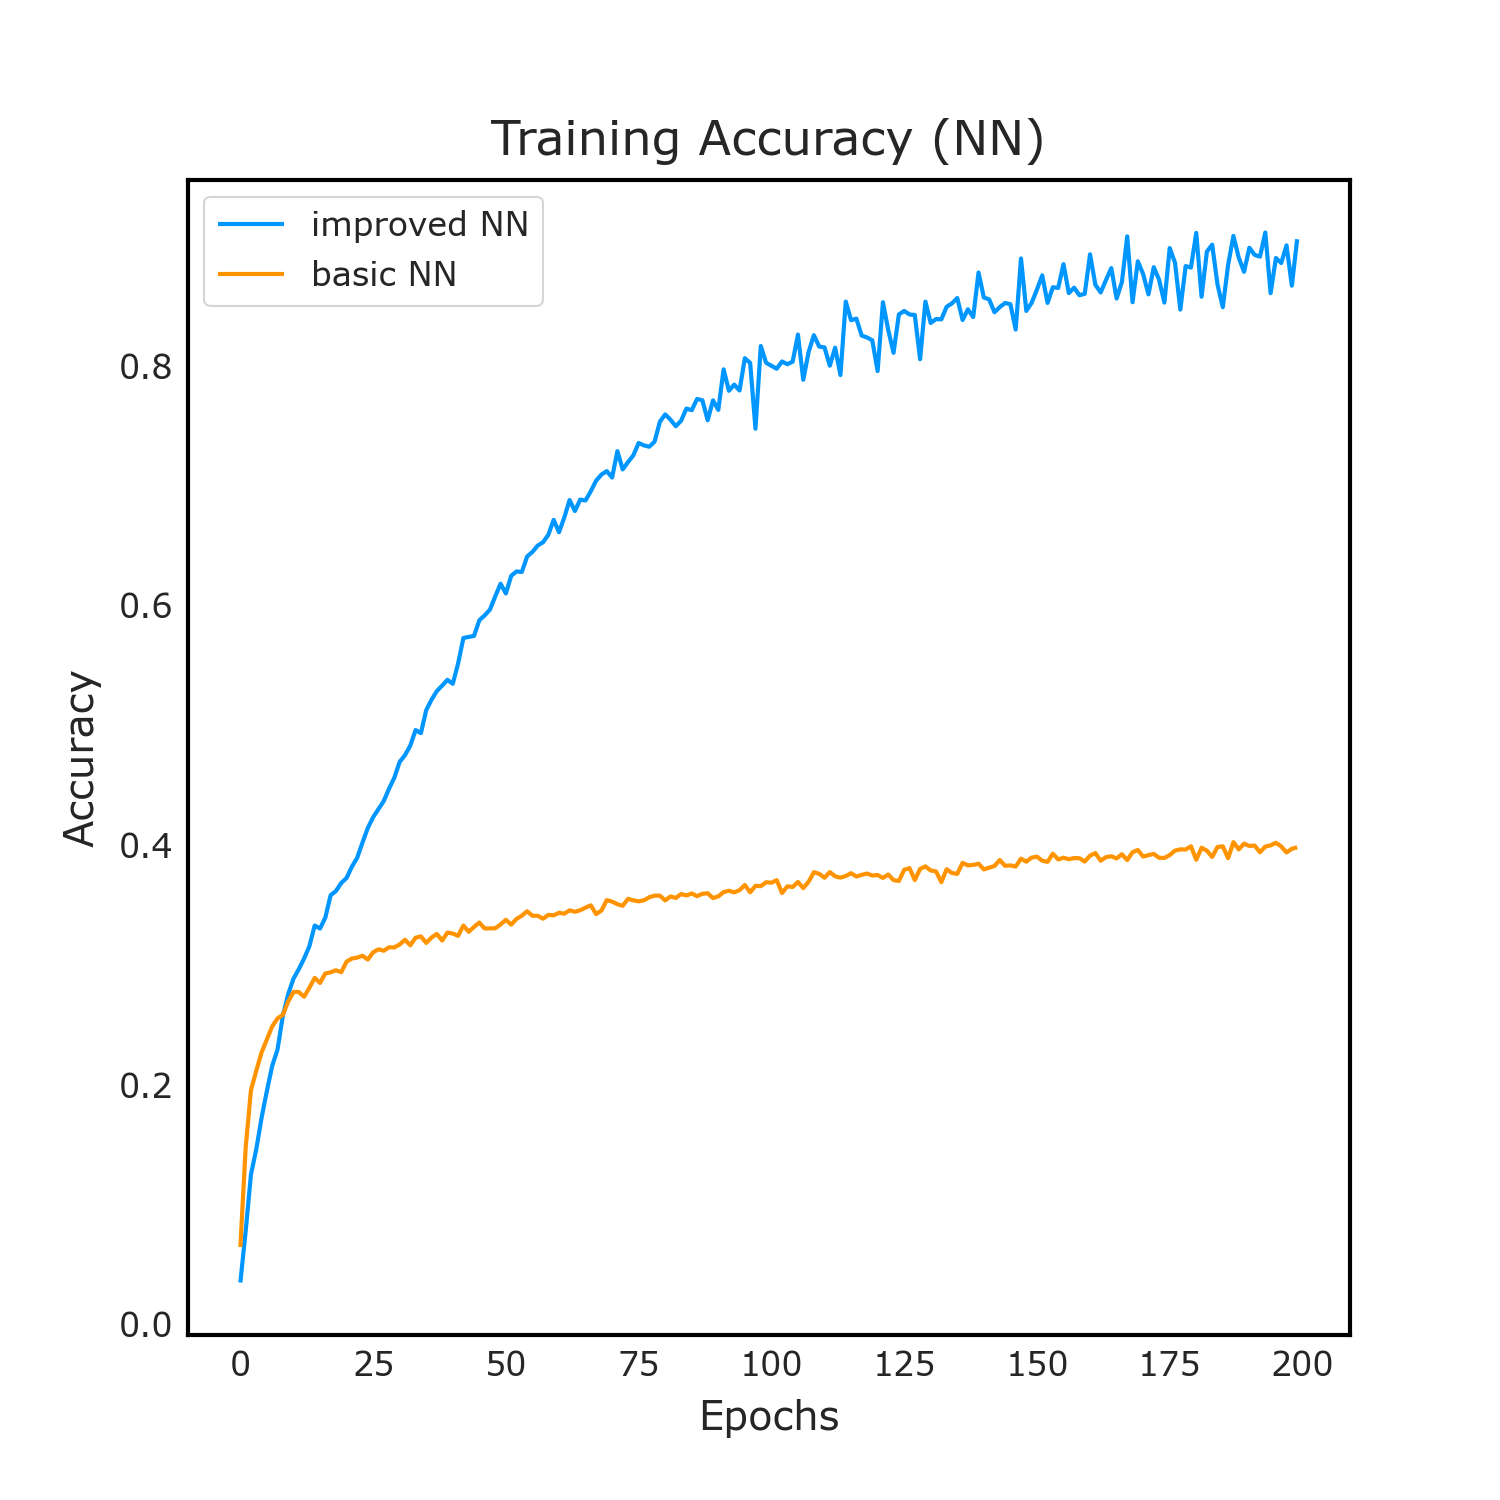
\includegraphics[width=\linewidth]{figs/train_accuracy.png}
        \caption{Training Accuracy per Epoch plot for Neural network}
        \label{fig:accuracy}
    \end{subfigure}%
    \begin{subfigure}{0.5\textwidth}
        \centering
        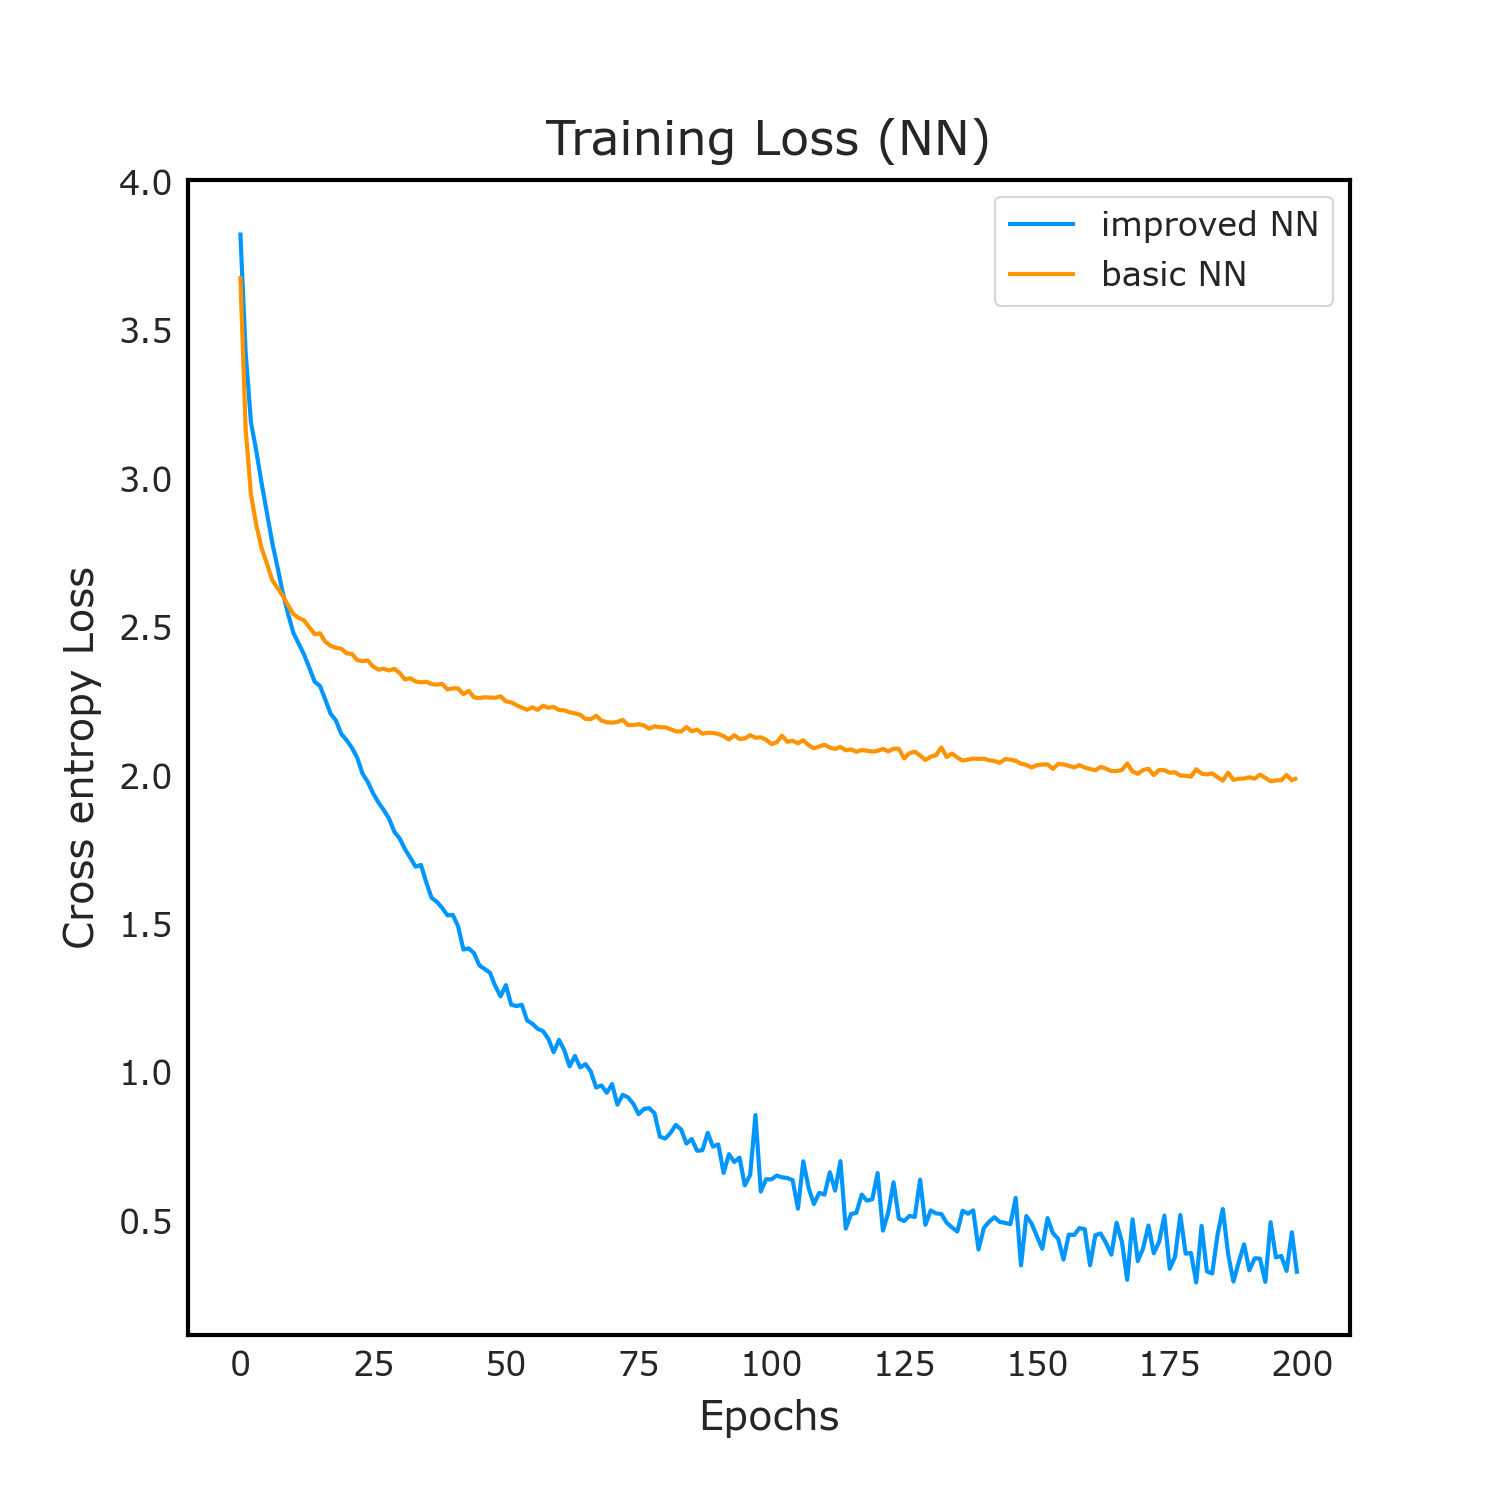
\includegraphics[width=\linewidth]{figs/train_loss1.png}
        \caption{Training Loss per Epoch plot for Neural Network}
        \label{fig:loss}
    \end{subfigure}
    \caption{Combined Figures}
    \label{fig:combined}
\end{figure}

\begin{figure}[h]
    \begin{subfigure}{0.5\textwidth}
        \centering
        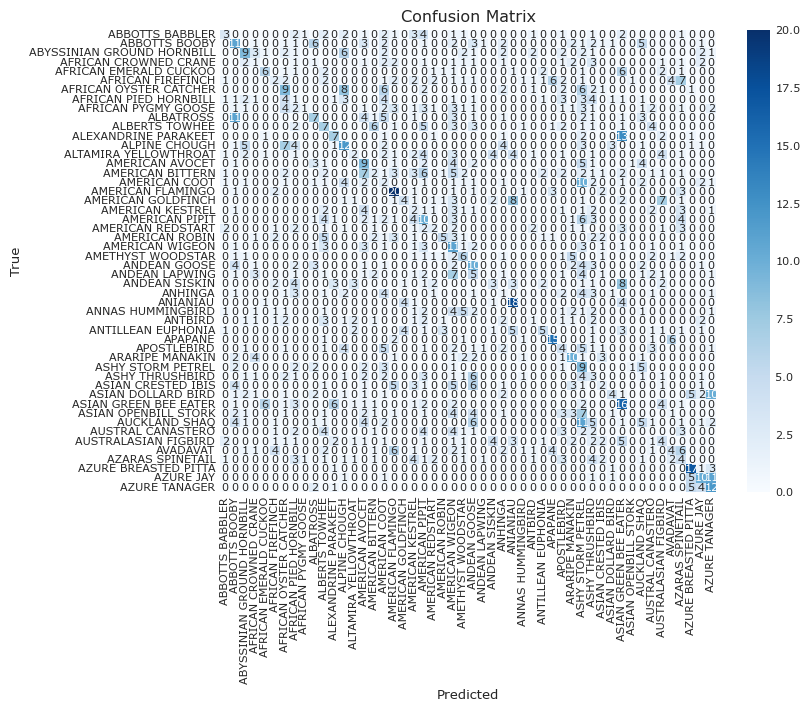
\includegraphics[width=\linewidth]{figs/matrix_baseline.png}
        \caption{Confusion matrix basic neural network}
        \label{fig:confusion basic}
    \end{subfigure}%
    \begin{subfigure}{0.5\textwidth}
        \centering
        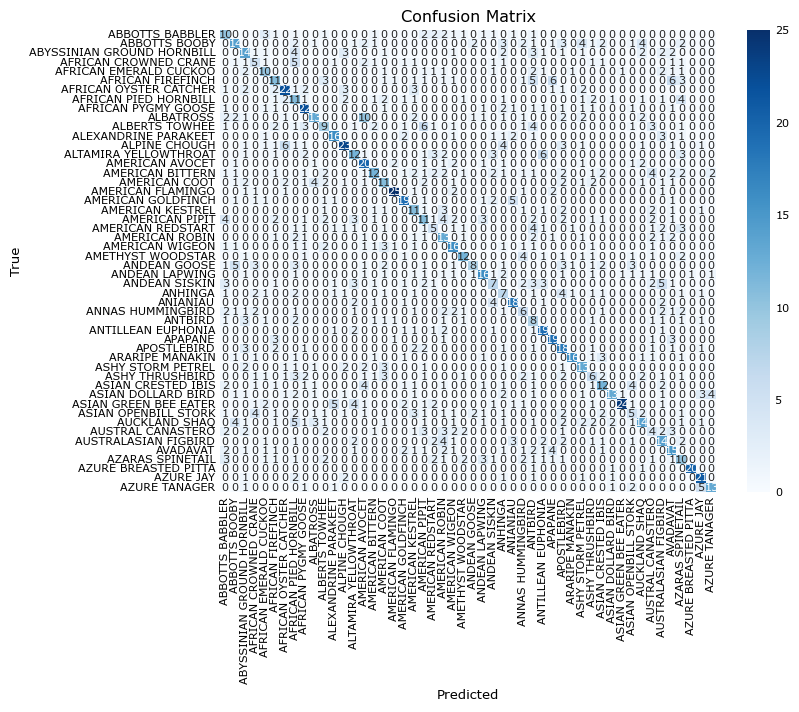
\includegraphics[width=\linewidth]{figs/matrix.png}
        \caption{Confusion matrix improved neural network}
        \label{fig:confusion improved}
    \end{subfigure}
    \caption{Combined Figures}
    \label{fig:combined}
\end{figure}
